\documentclass[runningheads,a4paper]{llncs}

\usepackage{amssymb}
\setcounter{tocdepth}{3}
\usepackage{graphicx}

\usepackage{url}
\urldef{\mailsa}\path|{pghilardi,ricardo}@inf.ufsc.br| \newcommand{\keywords}[1]{\par\addvspace\baselineskip
\noindent\keywordname\enspace\ignorespaces#1}

\begin{document}

\mainmatter  % start of an individual contribution

% first the title is needed
\title{SEA/Aspect: Dynamic Visualization and Composition of Concerns in Aspect-Oriented Modeling (AOM)}

% the name(s) of the author(s) follow(s) next  NB: Chinese authors should write their first names(s) in front of their surnames. This ensures that the
% names appear correctly in the running heads and the author index.
\author{Pedro Ghilardi, Ricardo Pereira e Silva}
%  (feature abused for this document to repeat the title also on left hand pages)

% the affiliations are given next; don't give your e-mail address unless you accept that it will be published
\institute{Federal University of Santa Catarina\\
Department of Informatic and Statistics\\
Florian�polis, Santa Catarina - Brasil\\
\mailsa\\
}

%  NB: a more complex sample for affiliations and the mapping to the corresponding authors can be found in the file "llncs.dem" (search for the string
% "\mainmatter" where a contribution starts).
% "llncs.dem" accompanies the document class "llncs.cls".

\maketitle

\bibliographystyle{splncs}

\begin{abstract}
The Aspect-Oriented Modeling (AOM) aims to raise the abstraction level from code
to models in the representation of aspect-oriented systems. With the modeling
of aspects it is possible to view the crosscutting concerns into the core
concerns of the system through the composition of models, which eases the
system comprehension. This paper aims at the representation of aspect-oriented
systems using UML, through a lightweight profile, modeling the most important features 
of Aspect-Oriented Programming (AOP) and enabling alternating views of the
system dynamics. The developer may create different compositions of the core and 
the crosscutting models, visualizing only the core models, the
crosscutting models, or the core intertwined with the crosscutting models. Aspects can be 
enabled or disabled dynamically, by updating the compound model, with no effort
demanded from the developer. The concerns are differentiated in the compound
model by different colors. The proposed solution is implemented as a tool, named
SEA/Aspect, that enables the automatic generation of sequence diagrams resulting from 
the intertwining of aspects, which also allows the selection of which aspects will be composed.
\end{abstract}

\keywords{Aspect-Oriented Modeling, UML, Model Composition, Model
Visualization, Model Weaving, Modeling Tool}

\section{Introduction}

A system consists of a set of requirements, where each requirement can be considered a customer{'}s concern. The core concerns captures the
core functionality and impact only a part of the system, while the crosscutting concerns captures functionality that impacts one or more
parts of the system. The AOP{'}s goal is the modularization of these concerns, so that they are kept in separate modules
that implement the core concerns of an application \cite{Laddad:2003:AAP:993468}.

The most elementary way to represent aspect-oriented programs is directly at the code level. One of the limitations of this approach is that the concerns
modularization makes it difficult to understand the execution flow, since the system dynamic is visualized only after the composition of concerns, or
with the aid of tools for visualizing the effect of the aspects in the system core. Another limitation of the direct implementation in code is that
with the low-level of abstraction, the developer may be overwhelmed with implementation details rather than on the interaction of the core and
crosscutting concerns. 

An aspect-oriented system demands the representation of the characteristics inherent to AOP and may have their understanding facilitated by
alternating the views of the application dynamic, visualizing the crosscutting concerns composed with the core concerns. As we
are working in the modeling of aspect-oriented applicatons, the model of a crosscutting concern will be referred as a crosscutting model and the model
of a core concern as a core model. The Unified Modeling Language (UML), the standard language used to model object-oriented systems \cite{uml:05},
could be used for aspect-oriented systems, but it have elements that cannot be represented with the standard meta-model. To overcome this limitation,
the language could be extended by two ways: via a lightweight extension through a profile, or an extension through the modification of the language
meta-model.

Some approaches have been proposed for the modeling of aspect-oriented systems using UML. A group of proposals extends the language meta-model
\cite{Kienzle:2009:AMM:1509239.1509252} \cite{theme:04} \cite{Klein:2007:WMA:1805812.1805819} \cite{Jacobson:2004:ASD:1062430}
\cite{Zhang:2012:WSA:2162049.2162080} introducing non-standard language constructs to represent the structure and behavior of aspect-oriented
applications. Another set of proposals extends the UML through a lightweight profile \cite{stein:02} \cite{Evermann:2007:MSP:1229375.1229379}
\cite{Cottenier06themotorola}, which can be used in CASE tools that support importing profiles. According to Fuentes \cite{fuentes-profile:1755547},
although each form of extension has its advantages and disadvantages, in most cases, the extension through a profile is better than extending the
meta-model, because the meta-model extensions cannot be used in CASE available tools. 

Our proposed approach specifies aspect-oriented software through a lightweight profile, using some stereotypes from the Evermann{'}s profile and
proposing others to represent the behavior of the core and crosscutting concerns. The constructions are based in the AspectJ language
\cite{AspectJ11}, which is the standard language for AOP with Java. Stein{'}s profile also allows the specification of aspect-oriented applications,
but we choose to extend the Evermann{'}s profile because it represents the most important characteristics of AOP, including the separation of concerns
in packages and the specification of the most important pointcut types. Our proposed approach overcomes one limitation of the Evermann{'}s work, that
does not allow capturing multiple join points with wildcards in the pointcut definition. In the Evermann{'}s approach, a pointcut refers to a specific
model element that must be explicitly specified by the modeler. Our approach represents pointcuts with states and transitions from the state machine
diagram. Each transition represents the capture of one or more join points, with the possibility of using wildcards. If the capture of all the join
points is satisfied, that is, if the conditions for triggering a transition are satisfied, it is considered that the system has met a certain
pointcut. The Cottenier{'}s proposal also uses the state machine diagram to represent pointcuts. However, the modeling is in a low-level of
abstraction with constructions close to the target language code. Our approach also differentiates from Cottenier{'}s in the modeling of advices.
While it models advices with the state machine diagram, we use the sequence diagram to represent the advices as a set of messages. In our approach,
the connection between pointcuts and advices is obtained with the use of state invariants, which are added in sequence diagrams. When the system mets
a pointcut, it enters in a state, this state is referred as a state invariant in the sequence diagram and triggers the execution of a set of messages,
that represents the advice behavior.

% Some approaches have been proposed for the modeling of aspect-oriented systems using UML. The Reusable Aspect Models (RAM)
% \cite{Kienzle:2009:AMM:1509239.1509252} approach represents the structure and the behavior of aspects, using class, sequence and state machine
% diagrams. The composed models generated by RAM are difficult to understand due to the excess of syntactic elements and because the core and
% crosscutting concerns are not explicitly differentiated in the compound model. Regarding to the language extension mechanism, RAM extends the UML
% meta-model by introducing non-standard language constructs, while this paper extends the UML through a profile. Cottenier{'}s paper
% \cite{Cottenier06themotorola} proposes an aspect visualization engine, with the representation of the AOP{'}s characteristics and the visualization of
% the effect of aspects in the system core, but with low-level of abstraction in the modeling and with constructions close to the target language code.
% Evermann{'}s proposal \cite{Evermann:2007:MSP:1229375.1229379} contributes with an AspectJ profile that represents most part of the AOP
% characteristics, but does not allow capturing multiple join points with wildcards. Klein{'}s approach \cite{Klein:2007:WMA:1805812.1805819} use
% extended sequence diagrams to model the system behavior and allows the composition of multiple aspects in the same joinpoint. However, the approach of
% Klein does not allow the representation of pointcuts with wildcards. Jacobson{'}s approach \cite{Jacobson:2004:ASD:1062430} represents aspects in
% terms of use cases, but modifies the UML meta-model by adding non-standard language constructs and does not perform automatic model composition.
% Theme/UML \cite{theme:04} supports the modeling of core and crosscutting concerns, automates the composition of models and represents the most important 
% features of AOP. Theme/UML modifies the UML meta-model and is dependent on the version 1.3 of the language. Carton{'}s proposal \cite{Carton:2009:MT:1692821.1692829} 
% aims to overcome this limitation, creating a marking profile to represent Theme/UML accordingly to the UML standards. However, the model composition is 
% still limited to the constructs available on the version 1.3 of the UML.

Using the constructions specified by the lightweight profile, this paper allows the automatic composition of core and crosscutting models, enabling
alternating views of the system dynamics (with and without the explicitation of the aspects) and, thus, facilitating the model understanding and
maintenance. A tool named SEA/Aspect, implemented in the SEA environment \cite{silva:00}, allows the dynamic enabling of aspects, visualizing only the behavior of the
core models, the crosscutting models, or the composition of one or more crosscutting models with a core model automatically. The developer differentiates the behavior 
of each concern by different colors in the compound model.

This article is organized as follows: section II presents the proposal for specification of aspect-oriented software. The section III deals with the
aspects composition and the visualization toggling tool. Section IV presents a case study using the proposed tool. The limitations are in the section V and 
the conclusions in the section VI.

\section{Specification of Aspect-Oriented Software}

Figure \ref{fig:full_profile} shows the UML profile to represent the structure and behavior of aspect-oriented applications. The profile may be used
in CASE tools that support importing profiles through the XML Metadata Interchange (XMI) \cite{xmi:11}. Relative to the structural modeling, this
paper uses some definitions from an AspectJ profile \cite{Evermann:2007:MSP:1229375.1229379}, which allows the representation of the AOP{'}s
structural characteristics. The definitions used from Evermann{'}s profile are the \textit{CrosscuttingConcern} and the \textit{Aspect} stereotypes,
that are colored in beige in the profile diagram. A stereotype extends an element from the UML meta-model improving its semantics.
In this paper, a meta-model element being extended will be represented inside parentheses. The \textit{CrosscuttingConcern} stereotype extends
(\textit{Package}) and contains a set of aspects and classes. It represents a concern that impacts one or more parts of the system. The
\textit{Aspect} stereotype extends (\textit{Class}), contains inter-type declarations and some configuration properties as:
type of aspect instantiation, associated pointcut and a flag to indicate if this aspect is privileged. Inter-type declarations allows injection of new
members (method, attribute) on a class, change of inheritance hierarchy and new interfaces implementation. To represent inter-type declarations, a new
stereotype denominated \textit{ClassExtension} was created. This stereotype extends (\textit{Class}) and is related to another stereotype named
\textit{Introduction}. The later is used to mark which member is being inserted on a given class, or which inheritance relationship is being added, or
which interface is being implemented. The stereotype \textit{Introduction} extends the meta-model elements (\textit{Attribute}), (\textit{Operation}),
(\textit{Generalization}) and (\textit{Realization}).

\begin{figure}[!h]
	\centering
	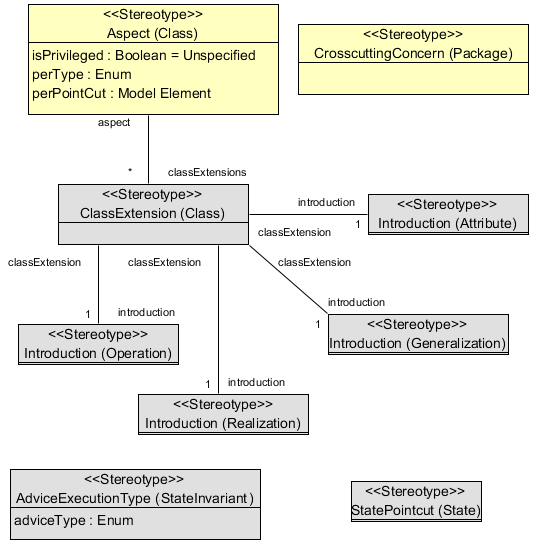
\includegraphics[scale=0.5]{img/full_profile.png}
	\caption{UML Profile to model Aspect-Oriented
	Applications.}\label{fig:full_profile}
\end{figure}

Besides inter-type declarations and aspect configurations, an aspect contains pointcuts and advices. Evermann{'}s profile
\cite{Evermann:2007:MSP:1229375.1229379} represents pointcuts within the aspect definition, but without the possibility of capturing multiple join
points, because it is not possible to use wildcards in the pointcut specification. In the Evermann{'}s approach, a pointcut refers to a specific model
element that must be explicitly specified by the modeler. This approach represents pointcuts with the UML state machine diagram. Each transition
represents the capture of one or more join points, with the possibility of using wildcards. If the capture of all the join points is satisfied, that
is, if the conditions for triggering a transition are satisfied, it is considered that the system has met a certain pointcut. The stereotype
\textit{StatePointcut} extends (\textit{State}) and represents a pointcut. The composition of pointcuts is achieved by composing different state
machines. The stereotype that represents pointcuts can be seen in the bottom right of figure \ref{fig:full_profile}.

The figure \ref{fig:pointcut_definition_1} shows the definition of pointcuts using the proposed approach. The pointcut \textit{AnyCall} captures calls
(\textit{call} pointcut) to any method of any class, using a wildcard to match any return type, any class and any method name with any number of
parameters. The pointcut \textit{RoomTarget} captures the occurences of a call when the target object (\textit{target} pointcut) is of the type
\textit{Room}. Each pointcut is represented as a state in the state machine diagram. The pointcut signature is specified in the transition, which
allows the use of wildcards to capture multiple joinpoints. When the pointcut state is reached, it means that the system has captured the execution
points specified by the pointcut signature in the transition label.

\begin{figure}[h]
	\centering
	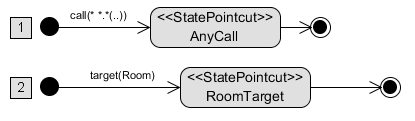
\includegraphics[scale=0.5]{img/pointcut_definition_1.png}
	\caption{The definition of two
	pointcuts.}\label{fig:pointcut_definition_1}
\end{figure}

The AspectJ language allows the composition of pointcuts with the logical operators \textit{and}, \textit{or} and \textit{not}. The proposed approach
performs the automatic composition of pointcuts using state machine digrams. The figure \ref{fig:pointcut_definition_and} shows the composition of the
pointcuts \textit{AnyCall} and \textit{RoomTarget} using the \textit{and} operator. The compound state machine contains a state with a
\textit{concurrent region}, containing sub-states that execute concurrently: \textit{AnyCall} and \textit{RoomTarget}. The synchronization occurs with
the \textit{fork} and \textit{join} nodes, which means that the final state (\textit{AnyCall AND RoomTarget}) only will be reached if both states
(\textit{AnyCall} and \textit{RoomTarget}) are reached. This is the semantic of the \textit{and} operator in the AspectJ language. The figure
\ref{fig:pointcut_definition_or} shows the composition of the pointcuts using the \textit{or} operator. Here the semantics is a bit different, because
the system will reach the final state (\textit{AnyCall OR RoomTarget}) when any of the pointcuts are reached. This is represented in the compound
state machine, that shows direct transitions from both states to the final state.

\begin{figure}[h]
	\centering
	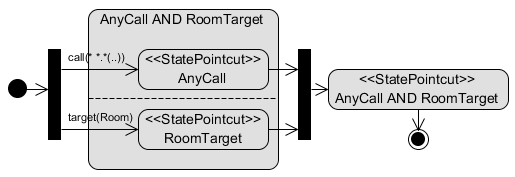
\includegraphics[scale=0.5]{img/pointcut_definition_and.png}
	\caption{The composition of two pointcuts
	with the AND operator.}\label{fig:pointcut_definition_and}
\end{figure}

\begin{figure}[h]
	\centering
	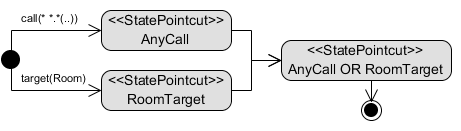
\includegraphics[scale=0.5]{img/pointcut_definition_or.png}
	\caption{The composition of two pointcuts
	with the OR operator.}\label{fig:pointcut_definition_or}
\end{figure}

A pointcut captures the execution points of a system to inject behavior in these points. This behavior is the advice, that is directly associated with
a pointcut. Sequence diagrams are used to represent the behavior of the core concerns (core model) and the crosscutting concerns (crosscutting
models). An aspect may have one or more advices and each one is represented by a crosscutting model. The behavior of an advice executes when it's associated
pointcuts are satisfied, i.e, all joint points are captured. As we model pointcuts with state machines and advices with sequence diagrams, the
connection of the advices with pointcuts should be achieved using syntatic elements of these diagrams. We implement this connection using state
invariants. A state invariant is an interaction fragment associated with a lifeline on the sequence diagram, representing a run-time constraint on the
participants of the interaction. We use the reachability of a state as the constraint to trigger the advice execution.

The definition of a crosscutting model (as a sequence diagram) begins
adding the aspect as the first lifeline of the diagram. A state invariant, which
represents the satisfaction of a pointcut, is associated to the aspect lifeline.
This means that the sequence of messages occurs only when the system achieves
the state pointcut represented by the state invariant. A stereotype named
\textit{AdviceExecutionType} is used to determine when the sequence of
messages will be performed: before, around or after the triggering of a 
pointcut. This stereotype extends (\textit{StateInvariant}) and can be viewed in
the bottom left of the figure \ref{fig:full_profile}.

The connection between advice and pointcuts can be better understood in the
example of the figure \ref{fig:behavioral_profile_example}. This figure shows
the pointcut previously specified to capture any method call on any class with
any numbers of parameters (\textit{AnyCall}). The log aspect defines a
crosscutting model that logs a message using a \textit{Logger}. The
crosscutting model is described as a sequence of messages in a sequence diagram. This diagram contains a state
invariant that refers to the \textit{AnyCall} pointcut. A state invariant must have the
advice execution type set as a tagged value to specify when the advice behavior
will be executed. In this example, the advice behavior will be executed 
\textit{after} the execution points captured by the \textit{AnyCall} pointcut.
The message \textit{log()} will be executed only when the state \textit{AnyCall} is achieved.

\begin{figure}[h]
	\centering
	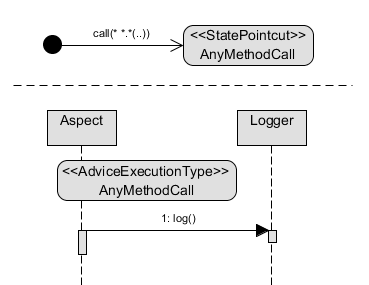
\includegraphics[scale=0.5]{img/behavioral_profile_example.png}
	\caption{The connection between
	pointcuts and advices using state
	invariants.}\label{fig:behavioral_profile_example}
\end{figure}

\section{AspectJ Pointcut Modeling}

This section shows the modeling of the most important pointcuts of the AspectJ
language.

\section{Composition and Visualization of Aspects}

The profile is added to the SEA environment \cite{silva:00}, which supports UML
diagramming. The SEA/Aspect is a tool which allows the selection of which 
crosscutting models will be intertwined together with the
core models of the system. One can automatically visualize only the core models, 
the crosscutting models, or core intertwined with crosscutting models. Aspects
can be enabled or disabled dynamically, by updating the compound model, with no 
effort demanded from  the developer. This automatic updating allows the toggling
of views, visualizing different model compositions. 

The SEA/Aspect has two different phases to output a compound model:
\textbf{selection} and \textbf{composition}. In the selection phase, the
developer selects the core and crosscutting concerns to compose. One or 
more aspects can be composed at the same time. The composition phase uses
wildcard matching and has the following steps:
  
	\begin{itemize}
	  \item \textbf{Match:} Find the execution points of the core model that are impacted by the
	  crosscutting models. This information is obtained from the pointcuts defined in the 
	  crosscutting models. The algorithm is separated in three steps:

	  \begin{enumerate}
	    \item \textbf{Find the pointcut:} To obtain the pointcut from the
	    crosscutting sequence diagram (crosscutting model), the algorithm looks for state invariants 
	    stereotyped as \textit{AdviceExecutionType}. This state invariants maps to
	    the state that defines the pointcut.
	    \item \textbf{Separate the pointcut:} The composer uses a regular
	    expression to separate a pointcut in four parts: \textbf{pointcut type}, \textbf{return type pattern},
	  \textbf{identification pattern} and \textbf{exception pattern}. 
	  The pointcut type is mandatory and is one of the types supported by the
	  AspectJ language, which includes \textit{execution}, \textit{call}, 
	  \textit{this} and others. The return type pattern is optional and specifies the return
	  type of the pointcut. The identification pattern is mandatory and contains
	  the signature to be matched in the core model. Finally, the exception pattern
	  is optional too, and is used to capture execution points that throws
	  exceptions of a given type
	    \item \textbf{Match the execution points:} This step starts using the
	  identification pattern to find the context information about the impacted 
	  concepts, like package and class context of a given method, for example. 
	  When all concepts inside a given context are captured, the algorithm uses
	  another regular expression to match the names of the captured concepts. 
	  For instance, when matching a method, the algorithm check return type,
	  parameters (name, type and number of parameters) and the method signature. 
	  Finally, the composer check for exception throws, if any. As output, the
	  concepts (classes and methods) impacted by the crosscutting models are
	  stored to be used in the merge activity.
	  \end{enumerate}  
	  
	  \item \textbf{Merge:} Merge concepts of the crosscutting models with
	  the impacted core model concepts. The merge receives as input the impacted
	  core model concepts that should be merged with croscutting ones. The merge
	  purpose is to inject a set of messages, lifelines, combined fragments and
	  other sequence diagram concepts in the core sequence diagram (core model),
	  adding new behavior defined in the crosscutting sequence diagrams
	  (crosscutting models). To achieve this, the algorithm is separated in
	  two steps:
		  \begin{enumerate}
		    \item \textbf{Find the advice type:} Retrieve the advice type from the
		    state invariant defined by the crosscutting model. The supported advice
		    types are: \textit{before}, \textit{around} and \textit{after}. The advice type gives the information of
		    when the messages should be injected in the core sequence diagram.
		  	\item \textbf{Inject the messages:} At this time, the algorithm knows the
		  	impacted concepts, the messages to inject from the crosscutting model 
		  	and when the messages should be inserted. The next
		  	step is the messages injection and reordering, because the injection of a
		  	message triggers a reordering event in the sequence diagram. With all
		  	the messages injected and ordered, the composer paints each message name
		  	with the correspondent crosscutting model color, to differentiate which
		  	message comes from which aspect. The merge produces as output a compound
		  	sequence diagram with the crosscutting concepts composed in the core
		  	sequence diagram.
		  \end{enumerate}
	  \end{itemize}  

\section{Case Study}\label{sec:case_study}

This section presents a case study to assess the applicability of the proposed
approach in the modeling of an application. The case study is based in the Hotel
Management System extracted from Jacobson{'}s book
\cite{Jacobson:2004:ASD:1062430}. This example allows the modeling of important
aspect-oriented funcionalities and is consolidated in the literature. The Hotel
Management System is composed by a set of use cases, like the check in and check out 
of customers, reservation of rooms, handling of a waiting list and a loyalty
program that allows the user to earn and redeem points.

The concerns represented in this case study are the following:

\begin{itemize}
  \item Check Out Customer: After the stay, the customer pays the bill
  and check out from the hotel.
  \item Earn Loyalty Points: The customer earns loyalty points after paying the
  bill.
\end{itemize}

  \begin{figure}[tb]
	\centering
	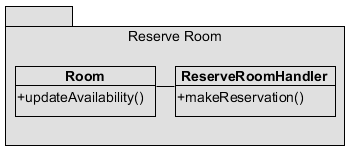
\includegraphics[scale=0.5]{img/case_study_structural_reserve_room.png}
	\caption{Case Study: Reserve
	Room Structural Model.}\label{fig:case_study_structural_reserve_room}
  \end{figure}
  
  \begin{figure}[tb]
	\centering
	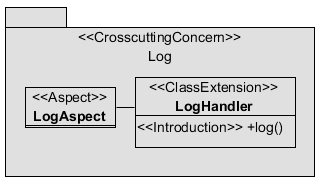
\includegraphics[scale=0.5]{img/case_study_structural_log.png}
	\caption{Case Study: Log Structural
	Model.}\label{fig:case_study_structural_log}
  \end{figure}

  \begin{figure}[tb]
	\centering
	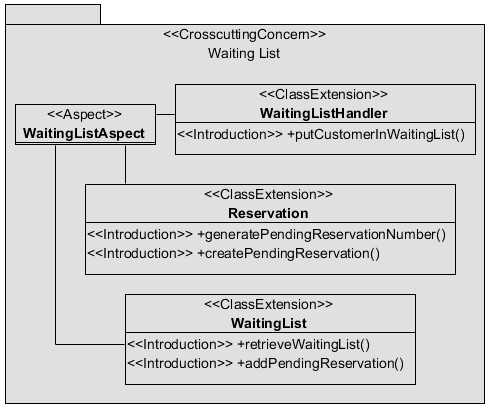
\includegraphics[scale=0.5]{img/case_study_structural_waiting_list.png}
	\caption{Case Study: Waiting
	List Structural Model.}\label{fig:case_study_structural_waiting_list}
  \end{figure}

The first concern being modeled is the reserve room functionality, that is a
system core concern and can be viewed in the figure
\ref{fig:case_study_structural_reserve_room}. As this is a core concern, it doesn't 
contains aspects neither class extensions, only classes to implement the concern. It has the
class \textit{Room} with the method \textit{updateAvailability()} and the class
\textit{ReserveRoomHandler} with the method \textit{makeReservation()}. The
crosscutting concern to log how many requests were done to a \textit{Room} is
modeled in the figure \ref{fig:case_study_structural_log}. It defines the
\textit{LogAspect} and one class extension named \textit{LogHandler}, that

  \begin{figure}
	\centering
	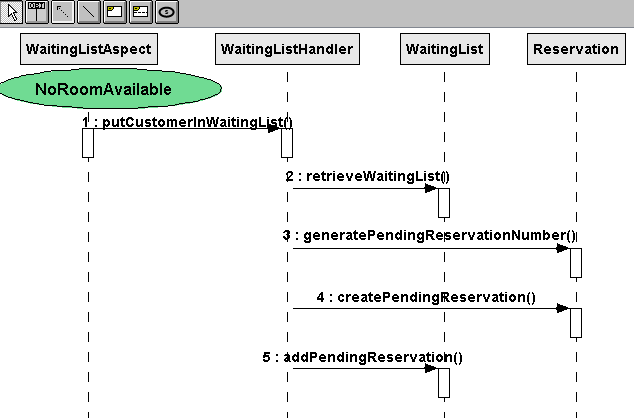
\includegraphics[scale=0.5]{img/waiting_list_behavioral_new.png}
	\caption{Case Study: Waiting List Sequence Diagram.}\label{fig:case_study_behavioral_waiting_list}
  \end{figure}

Finally, we have the crosscutting concern to handle waiting list in the figure
\ref{fig:case_study_structural_waiting_list}. The structural model of this
concern defines the \textit{WaitingListAspect} and three class extensions (with
some introductions). The first one is the \textit{WaitingListHandler}, that is
the controller between the system and the waiting list, the second adds methods to 
the \textit{Reservation} class to create reservations and the later is the
\textit{WaitingList}, that contains the pending reservations.

The models presented until now represents only the structure of the concerns,
which is not sufficient to understand the system as a whole. We need to
represent the system{'}s dynamic too. Sequence diagrams are used to represent
the behavior of core and crosscutting concerns, using the profile and the
process proposed by this approach. The modeling of concerns using behavioral
diagrams gives subsidies to achieve the toogling of views, that allows better
understanding of aspect-oriented applications, visualizing the effect of the 
aspects in the system.

We start with the sequence diagram of the reserve room concern, that can be
viewed in the figure \ref{fig:case_study_behavioral_reserve_room}. In a room
reservatiom, if the room isn't available, an exception is raised in the method
\textit{updateAvailability()}, otherwise, the reservation is done and the
customer receives a confirmation code.

  \begin{figure}[tb]
	\centering
	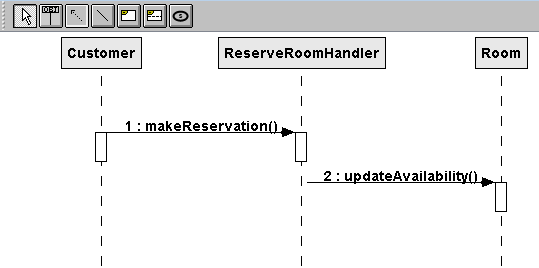
\includegraphics[scale=0.5]{img/case_study_behavioral_reserve_room.png}
	\caption{Case Study: Reserve Room Behavioral
	Model.}\label{fig:case_study_behavioral_reserve_room}
  \end{figure}
  
The other concerns to be modeled are the crosscutting concerns, that contains
pointcuts and advices. The log concern needs to account the number of requests to a room.
To achieve this, we define a pointcut that captures the calls to the
\textit{Room} class. This pointcut is modeled using the state machine diagram
and can be viewed in the figure \ref{fig:case_study_behavioral_pointcut_log}.

  \begin{figure}[tb]
	\centering
	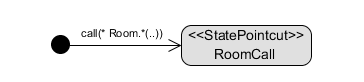
\includegraphics[scale=0.5]{img/case_study_behavioral_pointcut_log.png}
	\caption{Case Study: Log
	Pointcut Definition.}\label{fig:case_study_behavioral_pointcut_log}
  \end{figure}


With the pointcut defined, we create the sequence diagram to the log concern.
The diagram can be view in the figure \ref{fig:case_study_behavioral_log} and
contains as the first lifeline the \textit{LogAspect}. Accordingly to the
proposed approach, an aspect in the sequence diagram must have a state invariant
associated, which is the trigger to execute the sequence of messages. In this
case, the state invariant \textit{RoomCall} is associated with the
\textit{LogAspect} and points to a pointcut previously defined in the state
machine diagram. The semantics here is that the sequence of messages will execute only when the pointcut is 
satisfied. The message to be executed when the pointcut is satisfied is a call 
to the method \textit{log()} of the \textit{Logger} class. It is important to be
aware of the advice execution type, that is defined as a tagged value in the state invariant. The
proposed approach supports three types of advice types: before, after or
around. In this case, the advice type is after, which means that the log
behavior will execute after any method call to the \textit{Room} class. The sequence diagram
contains a combined fragment of type optional, that defines that the log only will be performed if the application is not
frozen. An application is not frozen when it is running in the
development environment. 

   \begin{figure*}
	\centering
	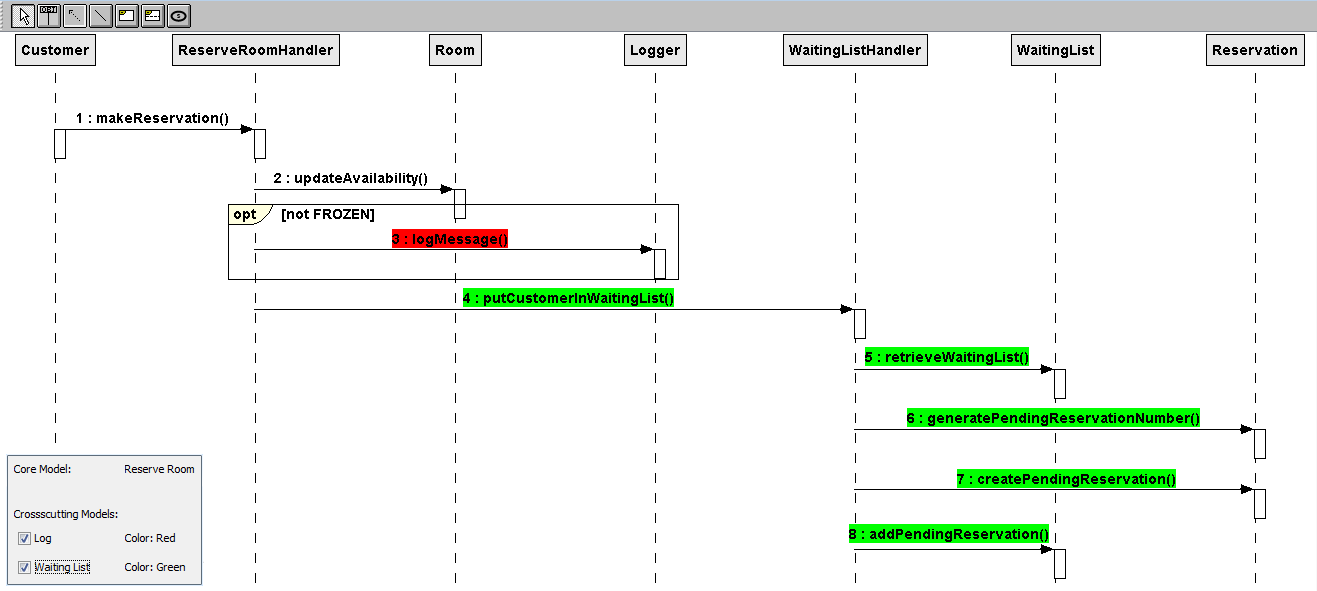
\includegraphics[scale=0.5]{img/case_study_compound_2.png}
	\caption{Case Study: Reserve
	Room composed with Log and Waiting List.}\label{fig:case_study_compound_2}
  \end{figure*}

The last concern to be modeled is the waiting list, that adds the customer to a
waiting list when a room isn't available. To achieve this, we need a pointcut
that captures when a customer try to reserve a room without success, because it
is unavailable. The pointcut in the figure
\ref{fig:case_study_behavioral_pointcut_waiting_list} captures calls to the
method \textit{updateAvailability()} of the \textit{Room} class, raising
the \textit{NoRoomsAvailable} exception.

  \begin{figure}[tb]
	\centering
	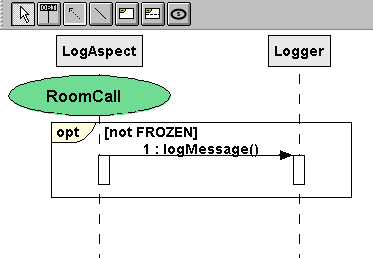
\includegraphics[scale=0.5]{img/case_study_behavioral_log.png}
	\caption{Case Study: Log
	Sequence Diagram.}\label{fig:case_study_behavioral_log}
  \end{figure}

  \begin{figure}[tb]
	\centering
	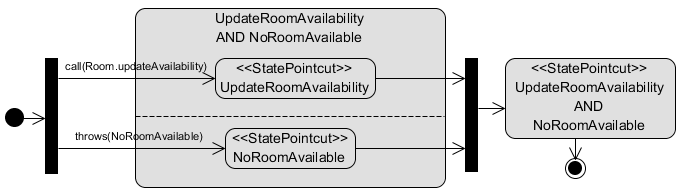
\includegraphics[scale=0.5]{img/case_study_behavioral_pointcut_waiting_list.png}
	\caption{Case Study Waiting List Pointcut
	Definition.}\label{fig:case_study_behavioral_pointcut_waiting_list}
  \end{figure}
  
Besides the pointcut definition, we need to define the behavior of how a
customer is added to the waiting list. This behavior is modeled in the 
sequence diagram of the figure \ref{fig:case_study_behavioral_waiting_list}. The
diagram has the \textit{WaitingListAspect} as the first lifeline and has a
sequence of messages to be executed when the system raises an exception that no rooms are 
available. These messages will be executed after the exception raising,
because the advice execution type of the state invariant is after.
  
After the structural and behavioral modeling of all the core and crosscutting
concerns, the modeler may interchange the model views, selecting which
concerns he wants to see composed in the same diagram. The SEA/Aspect tool
allows the selection of more than one model to be composed at the same
time. The figure \ref{fig:case_study_compound_2} shows a compound
model, with the concerns of reserve room, log and waiting list composed
together. The compound diagram shows the model selector in it is right bottom, that 
allows changing the models that are being show. The messages of different concerns are 
painted with different colors, as each concern has a color associated with it. 
This is useful to differentiate which messages comes from which aspect in the
compound model.
  
\section{Conclusion}

This work has proposed an approach to model aspect-oriented systems using UML,
with a specific profile that allows to implement an aspect visualizer in
the SEA environment. The SEA/Aspect tool performs the composition between core
and crosscutting models automatically, allowing the visualization of the aspect
dynamics in a system.

The main advantages of the proposed approach in relation to the others are: the
representation of all the characteristics of AOP, like the capture of multiple
join points with the representation of the aspect behavior; the definition of a
profile within the UML standards, which can be added in any CASE tool and the composition and
automatic visualization of the effect of the aspects in the core models in the
SEA environment, facilitating the understanding and maintenance of aspect-oriented
systems.

\bibliography{document}

\end{document}